\documentclass{article} 
\usepackage[utf8]{inputenc}
\usepackage{subcaption}
\usepackage[section]{placeins}

\title{CIS 510 Computer Vision - Project Proposal:\\
	Faking COVID-19: Fooling diagnosis with Normalizing flows} 
\author{Guzman, Luis and Walton, Steven}
\date{April 2020}

\usepackage{natbib} 
\usepackage{graphicx} 
\usepackage{amsmath} 

\begin{document}
\maketitle

\section{Part1}
The work for part 1 contained within the code `part1.py'. 
Note: Updates are in section~\ref{sec:updates}.

\begin{figure}
\centering
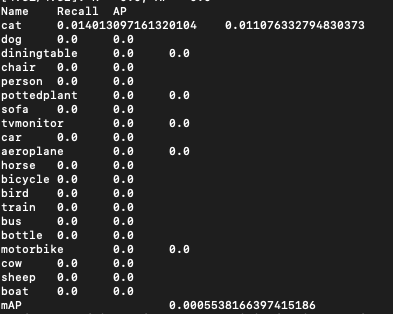
\includegraphics[width=\textwidth]{mAP.png}
\caption{Precision scores for classes after retraining network}
\end{figure}

\begin{figure}
\centering
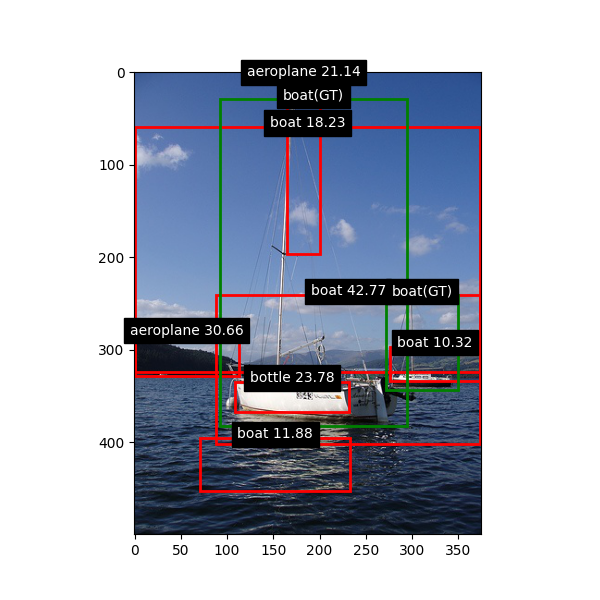
\includegraphics[width=\textwidth]{example.png}
\caption{Sample plot with ground truth labels in green}
\label{fig:boat}
\end{figure}

\begin{figure}
\centering
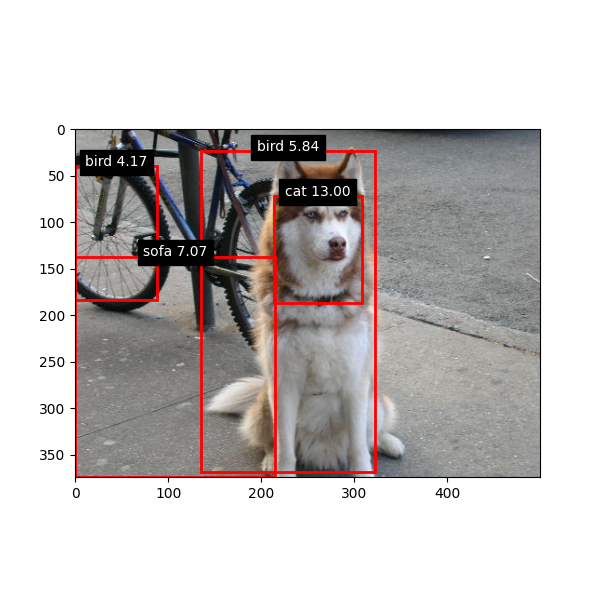
\includegraphics[width=\textwidth]{prevExample.png}
\caption{Sample plot without ground truth labels}
\label{fig:dog}
\end{figure}

\subsection{Analysis}
It appears that my network did not retrain well. If I had more time I would
adjust the network more so that we get better classification. I had trained
several times, dropping the learning rate as I went, and results were improving.
I suspect that dropping the learning rate even more would improve the results
even more. I had been fighting with COLAB for a few days where my simulation was
constantly hanging and running out of resources when processing a single image
and decided to move to another machine. This allowed me to improve results, but
made me already late on the assignment, so I cut my losses. 

Previous training gave a mAP score of 0, so they were not included. Still, the
score is still quite small here with a mAP of 0.0005. This looks like it is not
only due to miss classification, but the bounding boxes. In
Figure~\ref{fig:boat} we can see that we correctly identified boat in the two
locations but that the bounding boxes are not great. In this image no bounding
box had an IoU $\geq$ 0.5 and thus the precision on boats was 0 here. In
Figure~\ref{fig:dog} we can see that there is a lot of misclassifications here.
Better retraining of the network would show an improvement in this score. We can
conclude that the low mAP score is due to both of these effects. 

\section{Part2}
The code for part 2 comes from modifying mmdetection and using their model zoo.
I had to preprocess the VOC dataset using their included tools. The train tool
allows one to select different models where I used SSD300 and Faster RNN R50 FPN
1x. The results can be seen in Figure~\ref{fig:ssd} and
Figure~\ref{fig:faster_rcnn}, respectively. Each performed much better than the
results in part 1. As can be seen from the results SSD300 performed slightly
better than Faster RCNN.

\begin{figure}
\centering
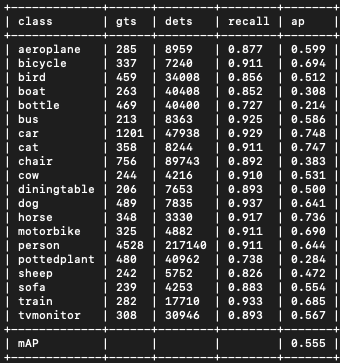
\includegraphics[width=\textwidth]{ssd300_voc07.png}
\caption{mAP results for SSD300}
\label{fig:ssd}
\end{figure}

\begin{figure}
\centering
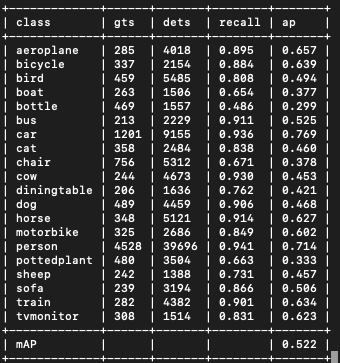
\includegraphics[width=\textwidth]{faster_rcnn_r50_fpn_1x_voc07.png}
\caption{mAP results for Faster RCNN}
\label{fig:faster_rcnn}
\end{figure}

\section{Extra Credit}
To perform part 1 I had to retrain the network so that it could properly use the
VOC labels. This code is included in the part1.py file under the function
``retrain".

\section{UPDATES}
\label{sec:updates}
Given the extra time I updated some of the parameters in the model and was able
to get a better mAP score. I changed the transform function and played around
with variables in the selective search. Both, as predicted originally, helped
give a better score. 

\subsection{Selective Search}
I did not measure directly the mAP scores for changes in the parameters. What I
did instead is selected a few images and investigated how the change in
parameters affected how accurately, under visual inspection, the search got the
objects we were looking for. The problem is to get the selective search to pick
up the large objects and not too small of objects. The biggest problem I was
having is that the search would select a bunch of small images and ignore the
large images that are closer to the ground truth. Maximal suppression helped
some, but there were a lot of squares with different classifications that made
this difficult. 

\subsection{Transfer function}
The transfer function the difference was that I used random resized crop and a
random horizontal flip. Previously I had just resized. The normalization
function is the same. Table~1 shows how different VGGs give
different mAP scores. Each of these trained for 20 epochs with a learning rate
of $10^{-4}$.

\begin{table}
    \centering
\begin{tabular}{|c|c|}
    \hline
    Model & mAP\\
    \hline
    VGG11 & 0.0107\\
    \hline
    VGG16 & 0.0112\\
    \hline
    VGG19 & 0.0114\\
    \hline
\end{tabular}
    \caption{mAP scores for different VGG models}
\label{models}
\end{table}

It can be seen that because we are better able to classify has a large change on
the mAP score. Figure~6 shows examples of how the different
models affects the accuracy. Most notably is the last image where only VGG19
correctly classifies the closeup image as a car. 

\begin{figure*}
    \centering
    \begin{subfigure}{\textwidth}
        \includegraphics[width=0.24\textwidth]{newTransform/vgg11/001394.png}
        \includegraphics[width=0.24\textwidth]{newTransform/vgg11/004238.png}
        \includegraphics[width=0.24\textwidth]{newTransform/vgg11/008545.png}
        \includegraphics[width=0.24\textwidth]{newTransform/vgg11/009963.png}
        \caption{VGG11}
        \label{fig:modela}
    \end{subfigure}
    \\
    \begin{subfigure}{\textwidth}
        \includegraphics[width=0.24\textwidth]{newTransform/001394.png}
        \includegraphics[width=0.24\textwidth]{newTransform/004238.png}
        \includegraphics[width=0.24\textwidth]{newTransform/008545.png}
        \includegraphics[width=0.24\textwidth]{newTransform/009963.png}
        \caption{VGG16}
        \label{fig:modelb}
    \end{subfigure}
    \\
    \begin{subfigure}{\textwidth}
        \includegraphics[width=0.24\textwidth]{newTransform/vgg19/001394.png}
        \includegraphics[width=0.24\textwidth]{newTransform/vgg19/004238.png}
        \includegraphics[width=0.24\textwidth]{newTransform/vgg19/008545.png}
        \includegraphics[width=0.24\textwidth]{newTransform/vgg19/009963.png}
        \caption{VGG19}
        \label{fig:modelc}
    \end{subfigure}
    \caption{Difference in VGG models}
    \label{fig:model}
\end{figure*}


\end{document}
